71. \begin{figure}[ht!]
\center{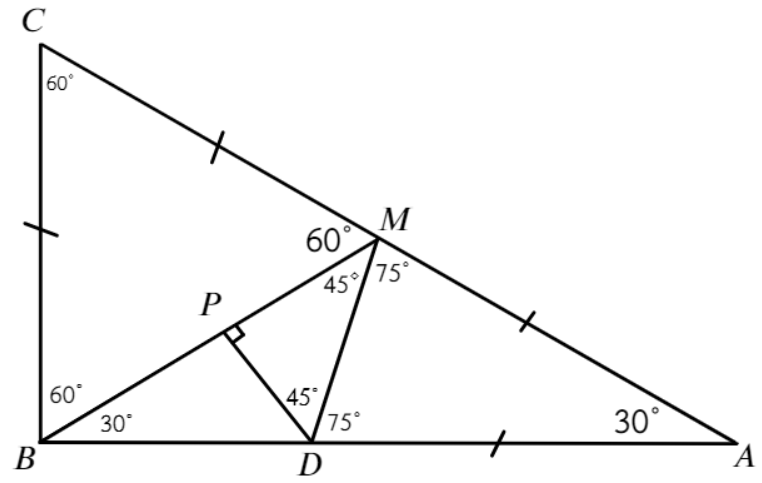
\includegraphics[scale=0.35]{g71.png}}
\end{figure}\\
Катет $BC$ лежит напротив угла в $30^\circ,$ значит $AC=2BC,$ поэтому $AM=\frac{1}{2}AC=BC=AD.$ Значит, треугольник $AMD$ является равнобедренным, а треугольник $BCM$ --- равносторонним ($BC=CM$ и $\angle C=90^\circ-\angle A=60^\circ.)$ Тогда $\angle DMA=(180^\circ-30^\circ):2=75^\circ,\ \angle PMD=180^\circ-60^\circ-75^\circ=45^\circ,\ \angle PDM=90^\circ-45^\circ=45^\circ,$ поэтому треугольник $PMD$ также является равнобедренным, $PM=PD.$ Найдём $\angle PBD=90^\circ-60^\circ=30^\circ,$ значит по теореме о катете, лежащем напротив угла в $30^\circ$ имеем $BD=2PD.$ Таким образом, $2P_{\Delta MDP}=2(PM+MD+PD)=
2PM+2MD+2PD=2PD+2PD+2MD=2BD+2MD=BD+MD+(BD+MD)>BD+MD+BM=P_{\Delta MDB},$ ч.т.д. ($BD+MD>BM$ по неравенству треугольника).\newpage
\noindent72. \begin{figure}[ht!]
\center{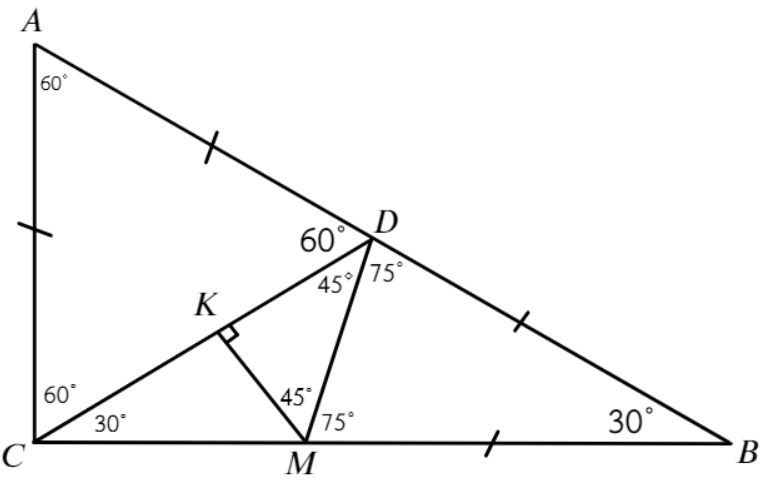
\includegraphics[scale=0.35]{g72.png}}
\end{figure}\\
Найдём $\angle B=90^\circ-60^\circ=30^\circ.$ Катет $AC$ лежит напротив угла в $30^\circ,$ значит $AB=2AC,$ поэтому $BD=\frac{1}{2}AB=AC=BM.$ Значит, треугольник $BMD$ является равнобедренным, а треугольник $ACD$ --- равносторонним ($AC=AD$ и $\angle A=60^\circ.)$ Тогда $\angle BDM=(180^\circ-30^\circ):2=75^\circ,\ \angle MDK=180^\circ-60^\circ-75^\circ=45^\circ,\ \angle DMK=90^\circ-45^\circ=45^\circ,$ поэтому треугольник $MDK$ также является равнобедренным, $KM=KD.$ Найдём $\angle KCM=90^\circ-60^\circ=30^\circ,$ значит по теореме о катете, лежащем напротив угла в $30^\circ$ имеем $MC=2KM.$ Таким образом, $2P_{\Delta MDK}=2(KD+MD+KM)=
2KD+2MD+2KM=2KM+2KM+2MD=2MC+2MD=MC+MD+(MC+MD)>MC+MD+CD=P_{\Delta DMC},$ ч.т.д. ($MC+MD>CD$ по неравенству треугольника).\\
